\documentclass{article}

% \usepackage[light]{merriweather} %% Option 'black' gives heavier bold face 
% \usepackage[default,regular,black]{sourceserifpro}
% \usepackage[T1]{fontenc}
\usepackage[T1]{fontenc}
\usepackage{ETbb}
\usepackage{amsmath}
\usepackage{amsfonts}
\usepackage{graphicx}
\usepackage{float}
\usepackage{tikz} 
\usepackage{filecontents}
\usepackage[style=verbose]{biblatex}

\usetikzlibrary {fit} 

\let\oldstylenums\textosf
\setlength{\tabcolsep}{26pt}

\title{Markov Random Fields (MRF)}
\author{Julien Burkhard}

\begin{document}

\maketitle

\section{Markov Chains}

In a first order Markov chain (MC):

\begin{align*}
	\Pr(X_i \mid X_{i-1}, X_{i-2}, \dots, X_1) = \Pr(X_i \mid X_{i-1})
\end{align*}

For example with:

\begin{figure}[!h]
\centering
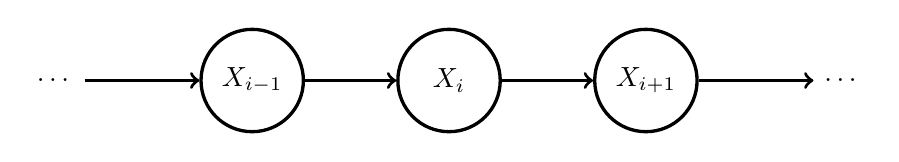
\begin{tikzpicture}[node distance={25mm}, very thick, 
	box/.style = {draw,very thick,inner sep=2mm,rounded corners=0mm},
	main/.style = {draw, circle, minimum size=13mm},
	rest/.style = {draw=none}] 
\node[rest] (0) {$\dots$};
	\node[main] (1) [right of=0]{$X_{i-1}$};
\node[main] (2) [right of=1] {$X_i$};
	\node[main] (3) [right of=2] {$X_{i+1}$};
\node[rest] (4) [right of=3] {$\dots$};
\draw[->] (0) -- (1);
\draw[->] (1) -- (2);
\draw[->] (2) -- (3);
\draw[->] (3) -- (4);
\end{tikzpicture} 
\end{figure}

For the sake of argument, let's consider $X_i \in \mathcal{F}_i$ as the event at time $i$ from the possible events $\mathcal{F}_i$. In all generality, we would expect for a causal process to simplify to:

\begin{align*}
	\Pr( X_i \mid \dots,X_{i+1},X_{i-1},\dots,X_1  ) = \Pr( X_i \mid X_{i-1}, X_{i-2}, \dots, X_1 ) 
\end{align*}

By Markov's property, it adds an additional constraint and says that:

\begin{align*}
	\Pr( X_i \mid X_{i-1}, X_{i-2}, \dots, X_{1} ) = \Pr( X_i \mid X_{i-1} )
\end{align*}

In other words, it is the \textbf{conditional independence} of $X_i$ w.r.t $X_{j}$ where $i\neq j$ but not the independence ! 

\begin{figure}[!h]
\centering
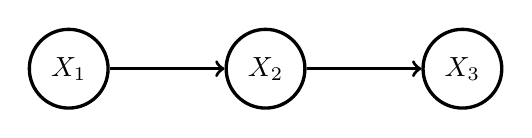
\begin{tikzpicture}[node distance={25mm}, very thick, 
	box/.style = {draw,very thick,inner sep=2mm,rounded corners=0mm},
	main/.style = {draw, circle, minimum size=10mm},
	rest/.style = {draw=none}] 
\node[main] (1) {$X_1$};
\node[main] (2) [right of=1] {$X_2$};
\node[main] (3) [right of=2] {$X_3$};
\draw[->] (1) -- (2);
\draw[->] (2) -- (3);
\end{tikzpicture} 
\end{figure}

As we can see for $X_1, X_2, X_3$.
\begin{align*}
	\Pr( X_3, X_1 ) &= \Pr( X_3 \mid X_1 ) \Pr(X_1)\\
	&= \Pr( X_3 \mid X_1 ) \Pr(X_1)\\
	&= \Pr(X_1) \sum_{X_2\in \mathcal{F}_2}\Pr( X_3 \mid X_2 ) \Pr( X_2 \mid X_1 ) \\
\end{align*}

Then independence is satisfied only if:

\begin{align*}
\Pr(X_3) = \sum_{X_2\in \mathcal{F}_2}\Pr( X_3 \mid X_2 ) \Pr( X_2 \mid X_1 )
\end{align*}

Which is not necessarily the case.
The following relation is used:

\begin{align*}
	\Pr( X_3 \mid X_1 ) &= \sum_{X_2\in \mathcal{F}_2}\Pr( X_3 \mid X_2 ) \Pr( X_2 \mid X_1 ) 
\end{align*}

Which is useful to express the dependence events to anterior events. More generally the event at state $i$ is dependent on the event $i-N$ with:

\begin{align*}
	\Pr( X_i \mid X_{i-N} ) &= \sum_{X_{i-2}\in \mathcal{F}_{i-2}, \dots, X_{i-N+1}\in \mathcal{F}_{i-N+1}}\Pr( X_{i-2} \mid X_{i-2} )\dots \Pr( X_{i-N+1} \mid X_{i-N} )
\end{align*}

So relating to algorithms and data structures,  the Markov chain formulation may be a instance of memoization to solve a Markov process joint probability !

\newpage
\section{Hidden Markov Model (HMM)}

The problem is as follows. We are given a series of observations $Z_i$ where there are hidden events $X_i$ modeled by a Markov chain. We may also have parameters for the model $\omega$. All of these are expressed through a probabilistic graph model such as this one:


\begin{figure}[!h]
\centering
\begin{tikzpicture}[node distance={25mm}, very thick, 
	box/.style = {draw,very thick,inner sep=2mm,rounded corners=0mm},
	main/.style = {draw,minimum size=10mm},
	rest/.style = {draw=none,minimum size=15mm}] 
\node[rest] (X0) {\dots};
	\node[main] (X1) [right of=X0] {$X_{i-1}$};
\node[main] (X2) [right of=X1] {$X_i$};
	\node[main] (X3) [right of=X2] {$X_{i+1}$};
\node[rest] (X4) [right of=X3] {\dots};
\draw[->] (X0) -- (X1);
\draw[->] (X1) -- (X2);
\draw[->] (X2) -- (X3);
\draw[->] (X3) -- (X4);

	\node[main] (Z1) [above of=X1] {$Z_{i-1}$};
\node[main] (Z2) [above of=X2] {$Z_i$};
	\node[main] (Z3) [above of=X3] {$Z_{i+1}$};

\draw[->] (X1) -- (Z1);
\draw[->] (X2) -- (Z2);
\draw[->] (X3) -- (Z3);

\node[main,black!30] (W) [above right of=Z2] {$\omega$};

\path[->,dashed,bend right, line,black!30] (W) edge (X1);
\path[->,dashed,bend left, black!30] (W) edge (X2);
\path[->,dashed,line,bend right, black!30] (W) edge (X3);
\path[->,dashed,bend right, black!30] (W) edge (Z1);
\path[->,dashed,line,black!30] (W) edge (Z2);
\path[->,dashed,bend left, line,black!30] (W) edge (Z3);

\end{tikzpicture} 
\end{figure}

Where we can express the likelihood of $\boldsymbol{Z}_N = \{ Z_1, \dots, Z_N \}$ w.r.t $\boldsymbol{X}_N = \{ Z_1, \dots, Z_N \}$ as:


\begin{align*}
	\Pr(\boldsymbol{Z}_N \mid \boldsymbol{X}_N) = \prod_{i}^{N} \Pr(Z_i \mid  X_i)
\end{align*}

The continous version of HMM is actually a Kalman filter !

\section{Markov Random Fields (MRFs)}

MRFs like MCs also define a conditional independence property:


\begin{align*}
	\Pr( X_i \mid \dots,X_{i+1},X_{i-1},\dots,X_1  ) = \Pr( X_i \mid	X_{j\in\mathcal{N}(i)}  ) 
\end{align*}

where $\mathcal{N}(i)$ is the set of events directly adjancent to $i$.

The joint probability which in MCs is computed on the last state is now defined as:

\begin{align*}
	\Pr( \boldsymbol{X} ) \propto \prod_{\boldsymbol{c}\in\mathcal{C}} \Pr( \boldsymbol{c} ) 
\end{align*}

Where $\mathcal{C}$ is the set of maximum cliques. This is the result of Hammersley-Clifford theorem.

Factor graphs makes which cliques are choosed explicit in the graph.

\end{document}
